\documentclass[a4paper]{article}

\usepackage[a4paper, total={5.5in, 9.5in}]{geometry}
\usepackage[english]{babel}
\usepackage[utf8]{inputenc}
\usepackage{amsmath}
\usepackage{graphicx}
\usepackage[colorinlistoftodos]{todonotes}
\usepackage{lipsum}
\usepackage[parfill]{parskip}
\usepackage[htt]{hyphenat}
\usepackage{titling}
\graphicspath{ {graphs/} }
\setlength{\droptitle}{-4em}
\title{COMP3204 - Scene Classification}

\author{
    Kwong Chi Tam\\
    \texttt{kcts1g13}
    \and
    Edward Cater\\
    \texttt{ec7g13}  
}

\date{\today}

\begin{document}
\maketitle

% -- IMPLEMENTATION DECISIONS --
\section*{Implementation Decisions}
We define classes Run1, Run2 and Run3, all of which inherit from a super class ``\texttt{Run}'' containing a number of useful fields and methods. This includes two  \texttt{GroupedDataset} instances for training and test data respectively, int variables \texttt{nTest} and \texttt{nTraining} to record the size of each data set (purely for more readable code) and some helper methods for loading/splitting data into training and test data sets. The descriptions for these methods can be found in the code comments.

\subsubsection*{Testing the Accuracy}
The labeled data provided by training.zip is randomly divided into training and set sets using \texttt{GroupRandomSplitter}. The training split is used to train the classifier and the test split is used to determine the accuracy.

\subsubsection*{Classifying Unlabeled Data}
Rather than splitting our data, all available labeled data from training.zip is used to train the classifier. The fully trained classifier is then used to make predictions on the unlabeled data from testing.zip, which is then written to a file.

\subsubsection*{On the Contributions of Team Members}
We took steps to ensure all three runs contained significant contributions from each team member. Ultimately, both team members contributed an equal amount of work.

\section{K Nearest-Neighbours}
For k nearest neighbor classification, first, each image is cropped about the center to a fixed resolution of 16 by 16 pixels. After cropping, the image is normalised and each row of pixels is concatenated into a float feature vector, where each element represents a single pixel’s normalised gray scale value (all images are grayscale by default). This is our “tiny-image” feature vector.

\subsection{Testing the accuracy of our classifier}

Feature vectors for training and test datasets are stored in separate, two dimensional float arrays; ``\texttt{trData[][]}'' and ``\texttt{tsData[][]}'', where each row corresponds to an image’s tiny-image feature vector. Both training and test set data have a corresponding array of strings; ``\texttt{trClass[]}'' and ``\texttt{tsClass[]}'' where each element is the class of the image represented by a row in \texttt{trData[][]} or \texttt{tsData[][]}.

An instance of OpenIMAJ’s \texttt{FloatNearestNeighboursExact} is created, which accepts \texttt{trData[][]} in its constructor. For every row in \texttt{tsData[][]}, we use the \texttt{FloatNearestNeighborsExact} object to retrieve a list of the nearest neighbors found in \texttt{trData[][]}, and a is prediction made according to the mode class from that list of neighbors. We compare the actual classification of that instance of training data against the prediction and record whether or not we are correct. Once a prediction has been made for all instances of training data, we calculate the accuracy. To tune this classifier, an average of five runs was computed for $k$ values ranging from 1-19 (Appendix - Figure 1). What was discovered that looking at only one neighbor resulted in the best classifier. Although this was still very low (approximately 21\% for $k=1$).

\subsection{Classifier Configuration}

\begin{center}
    \def\arraystretch{1.5}% 
    \begin{tabular}{ | l | r |}
    \hline
    \textbf{Variable} & \textbf{Value} \\ \hline
    k & 1 \\ \hline
    \end{tabular}
\end{center}
\bigskip

% -- DENSE PATCH SAMPLING --
\section{Dense Patch Sampling}
In order to implement a linear classifier using the \texttt{LiblinearAnnotator}, we designed our own feature extractor that made use of a custom engine, which is responsible for sampling and normalising 8x8 patches every 4 pixels in the x and y directions. The engine inherits from OpenIMAJ’s Engine class and overrides the \texttt{findFeatures()} method. This returns a \texttt{LocalFeatureList} of \texttt{FloatKeypoints}. To construct these \texttt{FloatKeypoints}, each row of pixels within in a patch are concatenated into a single row feature vector and passed to the \texttt{FloatKeypoint} constructor along with the position of the feature. Rather than returning all the features found by the engine, the \texttt{findFeatures()} method returns a subset of key points, obtained by random selection.

The \texttt{FeatureExtractor} requires the use of a \texttt{HardAssigner} in order to generate the bag-of-visual-words. This extracts features from the densely sampled pixel patches and uses K-Means to cluster them into separate classes. Initially, the suggested number of $\sim500$ clusters was used, however after testing the classifier with different numbers of clusters, it was found that using $\sim600$ clusters maximized the accuracy.

Once the \texttt{HardAssigner} has been trained, the \texttt{FeatureExtractor} uses a  \texttt{BlockSpatialAggregator} to append together the spatial histograms computed from the collection of visual words. The result of this is normalized and returned in the form of a feature vector.

\subsection{Testing the accuracy of our classifier}
An instance of \texttt{LiblinearAnnotator} is constructed using the custom feature extractor and trained using a subset of the images from training.zip data set. Internally, the data set is converted to a list containing exactly one reference to each object in the data set with (potentially) multiple annotations. 

The annotator is passed to a \texttt{ClassificationEvaluator}. Calling its evaluate method retrieves the predictions in the form of a Map, and calling its analyze method calculates the accuracy and error of the classifier.

This classifier required extensive training and tuning due to the number of parameters that can be changed. Because it is so computationally expensive, the training phase can take anywhere between 15-30 minutes and therefore only a small subset from the training.zip was split into training and testing data sets. Specifically, only 5 out of the 15 scenes were used for our tuning purposes, retrieving 50 images per group for the training set and 10 images per group for the testing set. It is worth noting that accuracy may seem higher than expected due to the smaller-sized data sets being used for tuning.\\

\begin{itemize}
\item The number of clusters was increased by 100 each time, but from our results (Appendix - Figure 2), we realised that having more than 600 clusters provided no valuable contribution to the accuracy.\\
\item After experimenting with different step sizes (Appendix - Figure 3), we found out that smaller values increased the accuracy of the classifier. However, this was payed with much slower performance speeds. Therefore, we considered a step size of 3 to be a reasonable balance between accuracy and performance.\\
\item The specification suggests to start by sampling 8x8 pixel patches, so we decided to increase the bin size to figure out what effect it would have on the overall accuracy (Appendix - Figure 4). The results show that there is no obvious pattern involving this parameter. However, using 14x14 pixel patches seemed to give the best accuracy.\\
\end{itemize}

\subsection{Classifier Configuration}
After training and tuning our classifier by modifying the mentioned parameters, we concluded that the following configuration is reasonable for our purposes, managing to achieve approximately 30\% accuracy on a training set composed of 90 images per group and testing set composed of 10 images per group.\\
\begin{center}
    \def\arraystretch{1.5}% 
    \begin{tabular}{ | l | r |}
    \hline
    \textbf{Variable} & \textbf{Value} \\ \hline
    Step size & 3 \\ \hline
    Patch size & 14 \\ \hline
    Number of clusters & 600 \\ \hline
    \end{tabular}
\end{center}
\bigskip

% -- PYRAMID DENSE SIFT WITH HOMOGENEOUS KERNEL MAP --
\section{Pyramid Dense SIFT with Homogeneous Kernel Map}
For the purpose of scene classification, using SIFT descriptors for patches within regular grid spaces has shown to be more suitable than descriptors of local interest points \cite{lazebnik2006beyond, fei2005bayesian}. Knowing this, we opted to use a dense SIFT engine to compute and describe a collection of 8x8 patches taken at a step size of 3 pixels. From the patches, a subset is taken by random selection, whose SIFT descriptors are used to generate visual bags of words. A \texttt{PyramidSpatialAggregator} is used rather than the \texttt{BlockSpatialAggregator} for computing the spatial histograms across the image. Additionally, by applying a homogeneous kernel map, the non-linearly separable data is projected into space where it can be analyzed by a linear classifier. This is a highly accurate approximation of applying a nonlinear classifier.

Rather than just using dense SIFT, this classifier makes use of spatial pyramid matching, which is regarded to be ``one of the most successful methods in computer vision''\cite{he2014spatial}. The \texttt{PyramidDenseSIFT} class within OpenIMAJ takes a normal \texttt{DenseSIFT} instance and applies it to different sized windows on the regular sampling grid.

The feature extractor for this classifier uses a \texttt{PyramidSpatialAggregator} to append the spatial histograms computed from the collection of visual words, returning the aggregated results in the form of a single vector. Unlike \texttt{SpatialBlockAggregator}, this approach groups the local features into fixed-size spatial blocks within a pyramid.

\subsection{Training and tuning}
The training process similar to the previous run. First, a \texttt{LiblinearAnnotator} is constructed by passing it a pyramid histogram of words extractor and then trained with a subset from the training.zip dataset. The \texttt{ClassificationEvaluator} from the OpenIMAJ library used to calculate the accuracy of the classifier.

Running the final classifier can take between 30-90 minutes depending on certain parameters. Because of this, we reduced the number of groups taken from training.zip, as well as the number images taken from each class significantly, from 90 and 10 (from the training and test set respectively), to just X and Y. With a reduced number of images, the time taken to run the classifier drops and multiple tests can be ran in succession, with variables adjusted slightly each time. By adjusting the variables with each run, the classifier can be tuned.\\

\begin{itemize}
\item Wrapping the \texttt{PHOWExtractor} with a \texttt{HomogenousKernelMap} improved the performance of our classifier significantly. Without it, accuracy was approximately 70\%, and applying the map sometimes improved the accuracy by up to 10\%.\\
\item Concatenating the spatial histograms using a \texttt{PyramidSpatialAggregator} rather than a \texttt{BlockSpatialAggregator} also had a positive impact on our classifier.\\
\item By varying the bin size scales for the \texttt{PyramidDenseSIFT}, we found out that using extra scales (e.g. 4, 6, 8, 10) provided a slight increase in performance compared to using a single window size. However, this meant that the time complexity of our classifier became much worse.\\
\end{itemize}

Using the training dataset, our classifier achieved a best-accuracy of roughly 80\%. The final run to produce the file of predictions took approximately 8.5 hours.

\subsection{Classifier Configuration}
Due to the extremely long running times of our classifier, we were not able to perform as much tuning as we had wished. However, we believe that our configuration allows our classifier to achieve an optimal accuracy.\\

\begin{center}
    \def\arraystretch{1.5}% 
    \begin{tabular}{ | l | r |}
    \hline
    \textbf{Variable} & \textbf{Value} \\ \hline
    Step size & 3 \\ \hline
    Patch size & 8 \\ \hline
    PyramidDenseSIFT scales & 4, 6, 8, 10 \\ \hline
    Number of clusters & 600 \\ \hline
    PyramidSpatialAggregator numBlocks & 2, 4 \\ \hline
    \end{tabular}
\end{center}

% --- APPENDIX ---
\newpage
\appendix

\section*{Appendix}

\bigskip
\bigskip

\begin{figure}[h!]
  \centering
  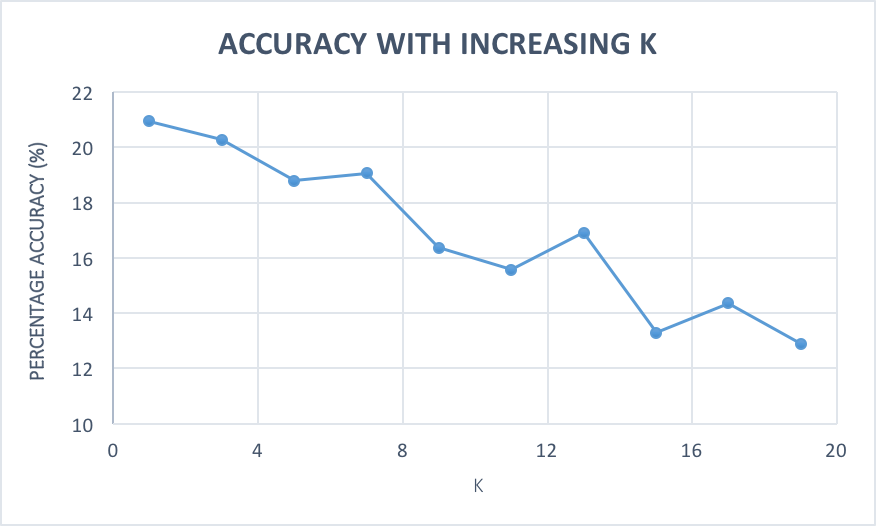
\includegraphics[width=1\textwidth]{kNN}
  \caption{Accuracy with increasing k}
\end{figure}

\bigskip \bigskip \bigskip \bigskip

\begin{figure}[h!]
  \centering
  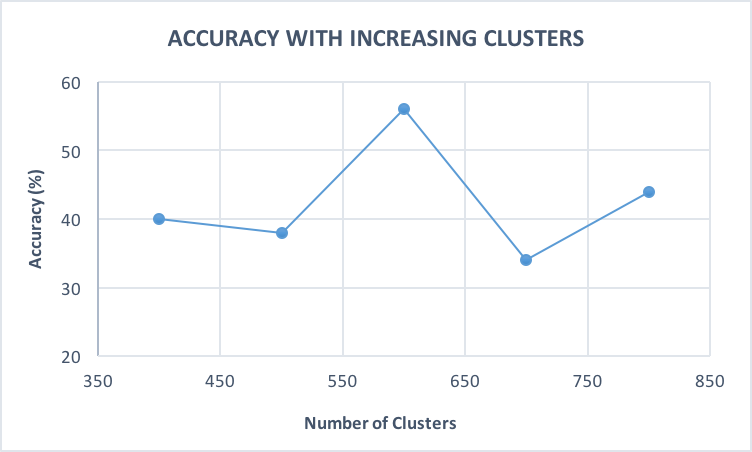
\includegraphics[width=1\textwidth]{clusters}
  \caption{Accuracy with increasing number of clusters}
\end{figure}

\begin{figure}[h!]
  \centering
  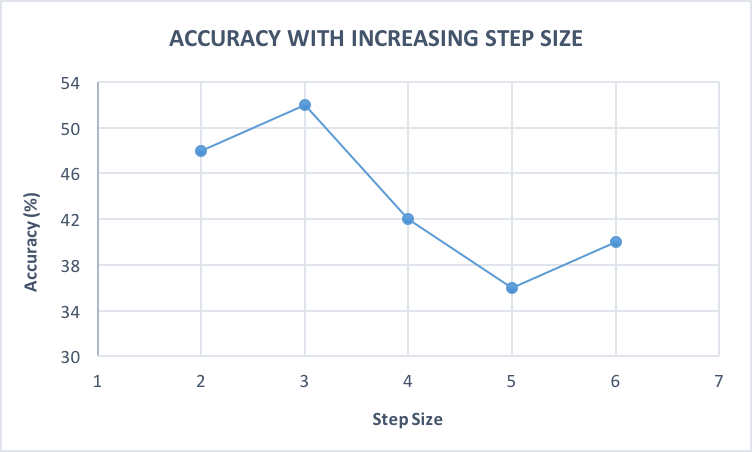
\includegraphics[width=1\textwidth]{step}
  \caption{Accuracy with increasing step size}
\end{figure}

\begin{figure}[h!]
  \centering
  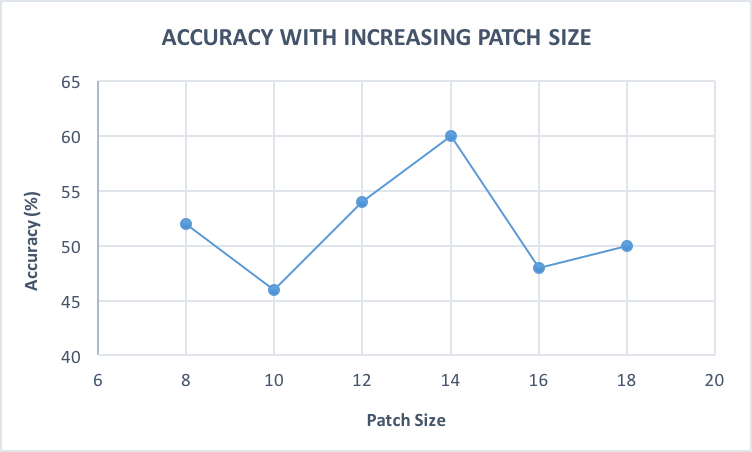
\includegraphics[width=1\textwidth]{patch}
  \caption{Accuracy with increasing patch size}
\end{figure}

% --- REFERENCES ---
\newpage
\clearpage
\bibliographystyle{plain}
\bibliography{sceneclassification_references.bib}
\end{document}